% !TeX root = ../main.tex
% Add the above to each chapter to make compiling the PDF easier in some editors.

\section{Content-Based Filtering}\label{section:content_based_filtering}

Content-based recommender systems employ features of both items and users to build item and user profiles that recommend items that are similar to the other items that the target user liked in the past. The necessary process of producing content-based recommendations consists of matching up the attributes of the target user profile, in which preferences and interests are stored, with the attributes of the items. After this process, we acquire a relevancy score that is an indicator for user-item relevancy. Generally, attributes that describe an item are features that are extracted from the item description. The content extracted from metadata is often too short and not sufficient to correctly define the user interests, that is why textual features are also added \cite{de2015semantics}.

\subsection{Overview of Content-Based Recommender Systems}

This section discloses an overview and the process of building a general content-based recommender system and the relevant techniques \cite{de2015semantics}.

The high level architecture of a content-based recommender system is shown in\ref{fig:high-level-content-based}. The recommendation process is performed in three steps, each of which is handled by a separate component \cite{de2015semantics}:

\begin{figure}[htp]
	\centering
	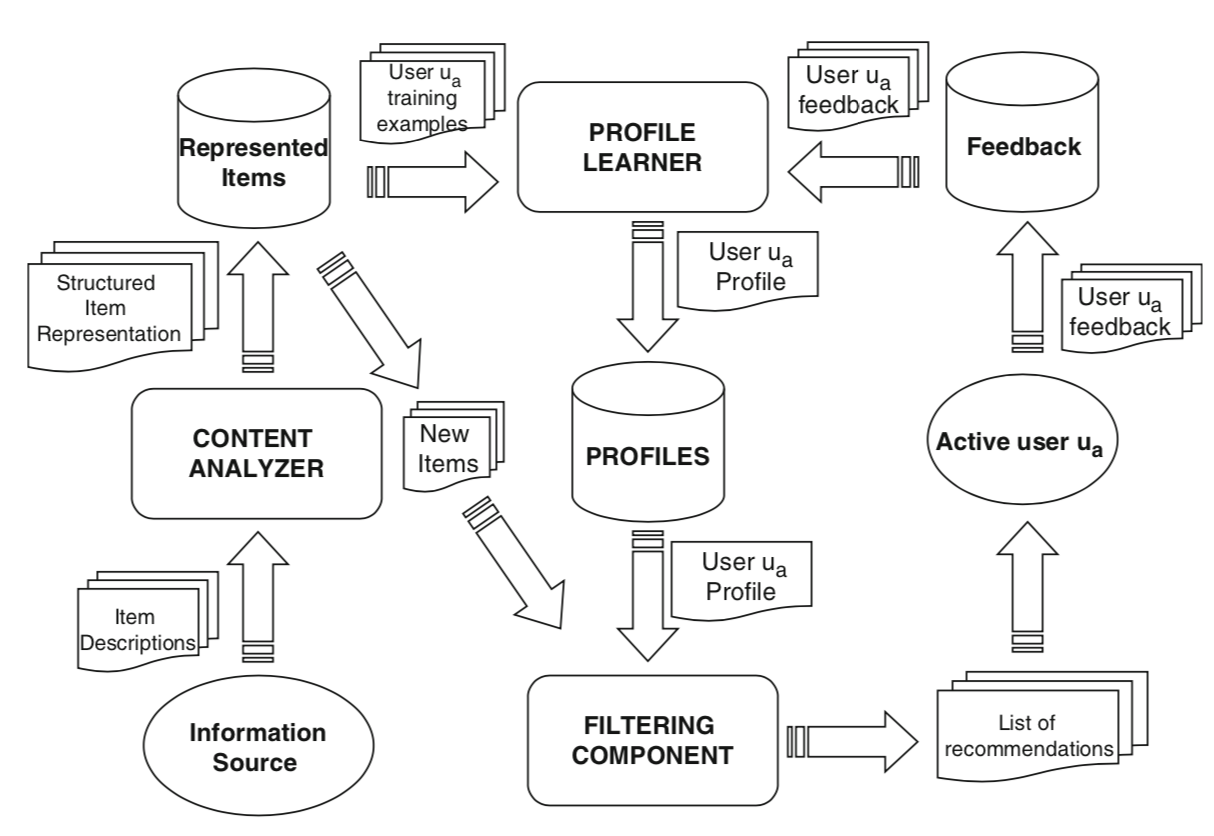
\includegraphics[width=\textwidth]{figures/HighLevelContentBased.png}
	\caption{High level architecture of a content based recommender  ~\parencite{de2015semantics}.}
	\label{fig:high-level-content-based}
\end{figure}



\begin{itemize}
	\item CONTENT ANALYZER—The first part of the architecture is responsible for scraping or getting the data from a source and saving them in a structured representation as items. If the data is a view data on a website, a scraper is needed to download and save them. However, if the desired input is metadata, then more advanced methods are needed to conduct an analysis. The output of this step is the input for the \textit{profile learner}.
	\item PROFILE LEARNER—The profile learner module gets the learning data and trains the model or creates the user profiles, which generalizes from the learning data. Using the generalization strategy, the profile learner creates a profile that improves on user's positive and negative interactions with the items. For the case of this thesis, we both create profiles for users and items(talents). The profile learner also takes advantage of enhancing the models with personal feedback after running on production mode.
	\item FILTERING COMPONENT—The last part of the architecture is the filtering component. It takes the user and item profiles, runs an operation, which generates a relevancy score for each user-item pair. Lastly, the component returns a recommendation list. Generating the relevancy score is a different process for different kind of models.
\end{itemize}

All of these components are crucial to make a functioning content-based recommender system. As the system always waits for new items, the feedback process is critical, and the retraining should happen regularly.


\subsubsection{Advantages and Drawbacks of Content-Based Filtering}

The advantages of content-based filtering against collaborative filtering are listed below \cite{de2015semantics}:

\begin{itemize}
	\item USER INDEPENDENCE—Content-based recommenders only need user profile for the relevant user. However, collaborative filtering recommenders require user profiles of all the other users so that it can suggest items based on nearest neighbors principle.
	\item TRANSPARENCY—Since the user profiles contain clear feature vectors, it is easy to directly understand why an item is recommended to a user by looking at their feature vectors. Conversely, collaborative systems are black boxes since the only explanation for an item recommendation is that unknown users with similar tastes rated that item positively.
	\item NEW ITEM—When a new item is added to the database, content-based recommendation systems can directly inject it to the system, because the feature vector of the new item is known. However, collaborative recommenders should wait until a substantial number of users rate this new item before the new item is recommended to anyone.
\end{itemize}

Nonetheless, content-based systems have drawbacks compared to collaborative filtering  \cite{de2015semantics}: 

\begin{itemize}
	\item LIMITED CONTENT ANALYSIS—To run content-based recommenders, feature vectors for items and users are created. However, the process of limiting content to feature vector loses information, or some misunderstandings can happen. For example, a popular machine learning library has two names: \textit{scikit-learn} and \textit{sklearn} or a popular frontend library is sometimes written as \textit{Vue} or \textit{Vue.js} or another popular programming language is called \textit{Python}, so is an animal and a TV show \textit{Monty Python}. Therefore, it is sometimes hard to create a \textit{perfect} feature vector of content.
	\item OVER-SPECIALIZATION — Since the content-based recommenders suggest items based on past behavior, they recommend items that are expected by the user. This drawback is also called lack of serendipity problem, which highlights the tendency of the content-based systems to produce recommendations with a limited degree of novelty. If a recruiter has only engaged with people who know Python, the recommender will also suggest people who know Python. A \textit{perfect} content-based technique would rarely find anything novel, limiting the range of applications for which it would be useful.
	\item NEW USER—Although it is easy to add new items to content-based recommender systems, it is not as easy to generate meaningful predictions for a new user. New users need to rate many items before we can recommend some items to them. This requirement means that the users need some history first so that the content-based recommenders work.
\end{itemize}


